\documentclass{beamer}
\usepackage[utf8]{inputenc} 
\usepackage[brazil]{babel} 
\usepackage{graphicx} 
\usepackage{amsmath, amssymb, amsfonts} 
\usepackage{color} 
\usepackage{lipsum}
\usepackage{float} 
\usepackage{multirow} 
\usepackage{url} 
\usepackage{hyperref} 
\usepackage{natbib} 
\usepackage{subfig}
\usepackage[default]{comfortaa}
\usepackage[T1]{fontenc}

\mode<presentation> {
	\usetheme{CambridgeUS}
    \usecolortheme{spruce}
}

\AtBeginSection[ ]
{
\begin{frame}{}
    \tableofcontents[currentsection]
\end{frame}
}

\title{Do Zero ao Julia}
% \subtitle{Semana da Computação 2022}
\author{João Víctor Costa de Oliveira} 
% A instituição irá aparecer na parte inferior dos slides.
\institute[] 
{
    \textit{}\\

	\medskip
	% Nome completo do departamento.
	\textit{}\\
    \medskip
}
% Data da apresentação
\date{2022} 


\begin{document}

\setbeamertemplate{blocks}[rounded][shadow=true]
% 1- Block title (background and text)
\setbeamercolor{block title example}{fg=white, bg=teal}
% 2- Block body (background and text)
\setbeamercolor{block body example}{ bg=teal!25}
% Change alert block colors
% 1- Block title (background and text)
\setbeamercolor{block title alerted}{fg=white, bg=purple}
% 2- Block body (background and text)
\setbeamercolor{block body alerted}{ bg=purple!25}
% Change standard block colors
% 1- Block title (background and text)
\setbeamercolor{block title}{bg=red, fg=white}
% 2- Block body (background)
\setbeamercolor{block body}{bg=red!10}


\begin{frame}
% Adiciona no primeiro slide as informações definidas anteriormente.
\titlepage
\begin{figure}[H]

\end{figure}
\end{frame}

\begin{frame}{Conteúdos abordados}
    % \footnotesize
    \tableofcontents
\end{frame}

\section{Histórico}
\begin{frame}{Introdução}
    \begin{itemize}
        \item Linguagem de programação
        \begin{itemize}
            \item Dinâmica
            \item Rápida
            \item Estruturada
            \item Compilada JIT
            \item OpenSource
        \end{itemize}
    \end{itemize}
\end{frame}

\begin{frame}{Introdução}
    \begin{itemize}
        \item Nascida em fevereiro de 2012
        \item Pensada para o uso em computação científica
        \item Criada para unir o melhor das linguagens
        \begin{itemize}
            \item Dinamismo do Ruby
            \item Notação matemática do Matlab
            \item Aplicado a estatísticas como o R 
            \item Simples como Python
            \item Rápido como C
        \end{itemize}
    \end{itemize}
\end{frame}

\begin{frame}{Introdução}{Filosofia Julia}
    \begin{block}{\centering FILOSOFIA JULIA}
        \centering
        \textbf{Ler como Python e rodar como C}
    \end{block}
\end{frame}

\begin{frame}{Introdução}{Empresas, instituições e projetos que usam Julia}
    \begin{itemize}
        \item INPE
        \item LAMPS - PUC Rio
        \item IBM \footnote{em um dos projetos no qual utilizam Julia, uma Rede Neural teve um aumento de velocidade de processamento em torno de $57\%$}
        \item MIT 
        \item CISCO
        \item BNDES
    \end{itemize}
\end{frame}

\section{Tipos de dados}
\begin{frame}{Tipos de dados}
    \begin{block}{Tipos de dados}
        Inteiro (10, -2, 4523, ...)\\
        Ponto flutuante (simples) (10.0, 4.6, 7.8954, ...)\\
        Complexo (4.5 + 3.78i = complex(4.5, 3.2)\\
        Booleanos (True, False)\\
        String (``abc'', ``Fluminense'', ...) 
    \end{block}
\end{frame}

\begin{frame}{Tipos de dados}{Tipagem de variáveis}
    \begin{itemize}
        \item Tipagem \begin{itemize}
            \item dinâmica
            \item forte
        \end{itemize}
        \item Variáveis não precisam ter o tipo declarado
        \item Quem cuida de atribuir um tipo para cada variável é o próprio compilador
    \end{itemize}
    \begin{figure}
        \centering
        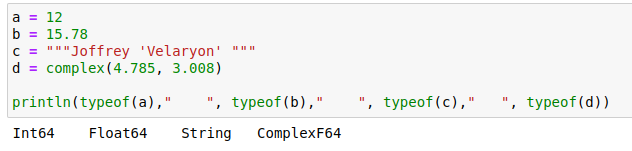
\includegraphics[scale=0.4]{imagens/tipos-variaveis.png}
        \label{fig:ex-tipos}
    \end{figure}
\end{frame}

\begin{frame}{Tipos de dados}{Tipagem de variáveis}
    \begin{itemize}
        \item Podemos ainda criar uma variável como \textcolor{blue}{inteiro}, e depois atribuí-la um valor \textcolor{purple}{float}, por exemplo
    \end{itemize}
    \begin{figure}
        \centering
        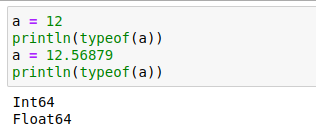
\includegraphics[scale=0.5]{imagens/tipagem02.png}
        \label{fig:ex-tipagem2}
    \end{figure}
\end{frame}

\begin{frame}{Tipos de dados}{Declaração de variáveis}
    \begin{itemize}
        \item Declaramos variáveis em Julia assim como declaramos em várias outras linguagens, usando o sinal de $``="$
        \item Ao contrário de linguagens como $C$ e $C$++, o ``;"  ao final de cada linha não é necessário
    \end{itemize}
    \begin{figure}
        \centering
        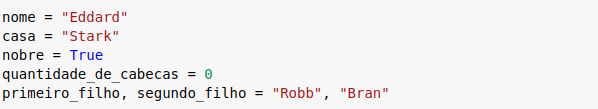
\includegraphics[scale=0.5]{imagens/declaracao-de-variaveis.png}
        \label{fig:declaracao-de-variaveis}
    \end{figure}
\end{frame}

\begin{frame}{Tipos de dados}{Declaração de variáveis}
    \begin{itemize}
        \item Julia nos permite escrever códigos super genéricos
        \item Podemos escrever um sistema todo nomeando as variáveis com emojis ou símbolos
        \item Isso pode ser interessante quando queremos escrever expressões por exemplo
        \begin{figure}
            \centering
            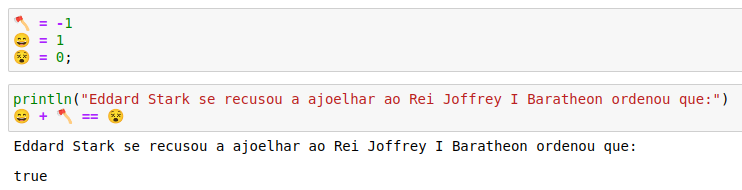
\includegraphics[scale=0.4]{imagens/ex-codigo-neutro.png}
            \label{fig:ex-tipos}
        \end{figure}
    \end{itemize}

\end{frame}

\begin{frame}{Tipos de dados}{Função de impressão}
    \begin{itemize}
        \item Utilizamos a função `` println() " para imprimir com quebra de linha ao final
        \item Utilizamos a função `` print() " para imprimir sem quebra de linha ao final
    \end{itemize}
    \begin{figure}
        \centering
        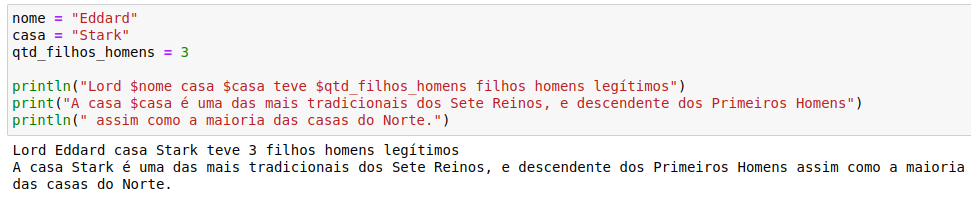
\includegraphics[scale=0.35]{imagens/ex-funcao-printar.png}
        \label{fig:ex-tipos}
    \end{figure}
\end{frame}

\begin{frame}{Tipos de dados}{Pegando valores do teclado}
    \begin{itemize}
        \item Usamos a função `` readline() " para ler um input do teclado
        \item Como para Julia tudo que vem do teclado é uma string, precisamos fazer um typecasting
        \item Para isso, usamos a função reservada `` parse() "
    \end{itemize}
    \begin{figure}
        \centering
        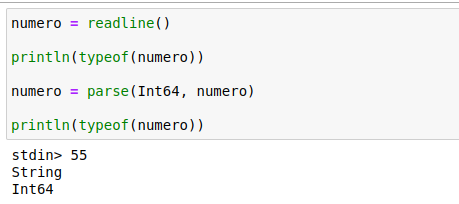
\includegraphics[scale=0.35]{imagens/ex-readline.png}
        \label{fig:ex-tipos}
    \end{figure}
\end{frame}

\begin{frame}{Tipos de dados}{Operações com variáveis numéricas}
    \tiny
    \begin{table}[]
        \centering
        \begin{tabular}{|c|c|c|c|}
            \hline
            \textbf{Operação} & \textbf{Sintaxe} & \textbf{Operação} & \textbf{Sintaxe} \\
             \hline \hline
            Adição & a + b & Valor absoluto & abs(a) \\\hline
            Subtração & a - b & Converter em inteiro & convert(Int64, variavel) \\\hline
            Produto & a * b & Converter em ponto flutuante & convert(Float64, variavel) \\\hline
            Divisão & a / b & Potenciação & a \^\ b \\\hline
            Divisão Inteira & a // b &  &  \\\hline
            Módulo & a \% b &  &  \\\hline
            Negação & - a &  &  \\\hline
        \end{tabular}
        \label{tab:tabela}
    \end{table}
\end{frame}

\begin{frame}{Tipos de dados}{Trabalhando com strings}
    \begin{itemize}
        \item Em Julia podemos inicializar strings de duas maneiras
    \end{itemize}
    \begin{figure}
        \centering
        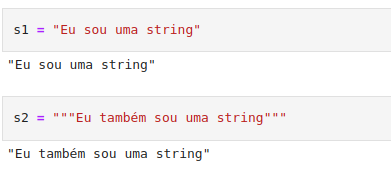
\includegraphics[scale=0.5]{imagens/strings01.png}
        \label{fig:my_label}
    \end{figure}
\end{frame}

\begin{frame}{Tipos de dados}{Trabalhando com strings}
    \begin{itemize}
        \item Geralmente usamos a segunda maneira quando precisamos colocar aspas dentro da string
        \item Isso pode ocorrer ao fazermos uma citação, por exemplo
    \end{itemize}
    \begin{figure}
        \centering
        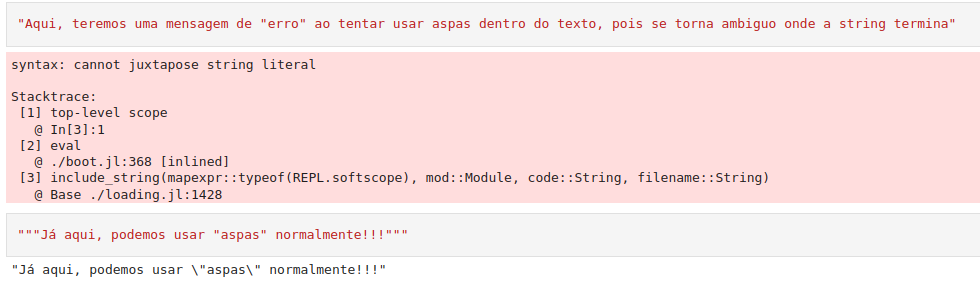
\includegraphics[scale=0.35]{imagens/string02.png}
        \label{fig:my_label}
    \end{figure}
\end{frame}

\begin{frame}{Tipos de dados}{Trabalhando com strings}
    \begin{block}{Atenção}
        Não confunda `a' com "a". Um é um \textcolor{blue}{caracter} e o outro é uma \textcolor{green}{string}
    \end{block}
    \begin{figure}
        \centering
        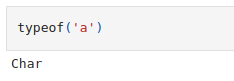
\includegraphics[scale=0.5]{imagens/char.png}
        \label{fig:my_label}
    \end{figure}
\end{frame}

\begin{frame}{Tipos de dados}{Interpolando strings}
    \begin{itemize}
        \item Podemos usar o sinal \$ para inserir variáveis existentes em uma string e avaliar expressões com a string
    \end{itemize}
    \begin{figure}
        \centering
        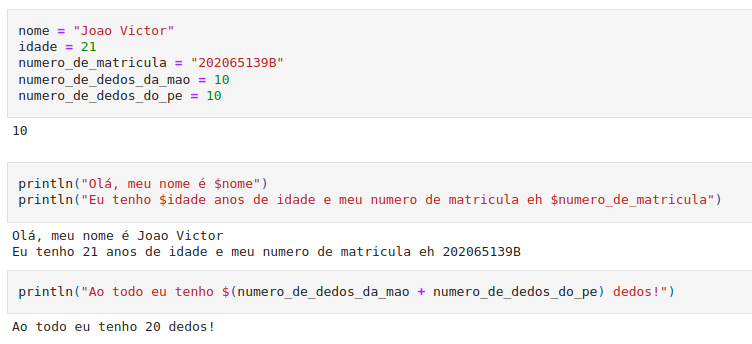
\includegraphics[scale=0.4]{imagens/string03.png}
        \label{fig:my_label}
    \end{figure}
\end{frame}

\begin{frame}{Tipos de dados}{Concatenação de strings}
    \begin{itemize}
        \item Vamos ver três maneiras de concatenar strings
        \item A primeira é usar a função string()
        \item string() também converte entradas ``não-string" em strings
    \end{itemize}
    \begin{figure}
        \centering
        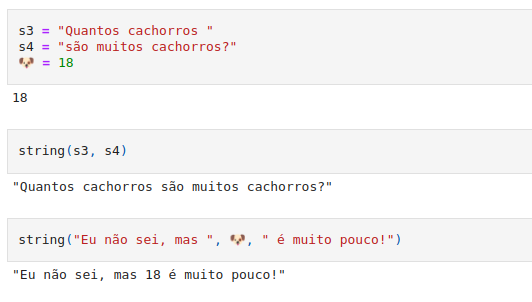
\includegraphics[scale=0.4]{imagens/string04.png}
        \label{fig:my_label}
    \end{figure}
\end{frame}

\begin{frame}{Tipos de dados}{Concatenação de strings}
    \begin{itemize}
        \item Também podemos usar * para concatenação
    \end{itemize}
    \begin{figure}
        \centering
        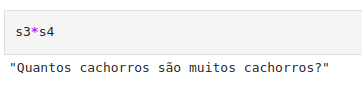
\includegraphics[scale=0.5]{imagens/string05.png}
        \label{fig:my_label}
    \end{figure}
\end{frame}


\section{Estruturas de Dados Básicas}
\begin{frame}{Estruturas de Dados}{Introdução}
    \begin{itemize}
        \item Vamos começar agora a trabalhar com Estruturas de Dados que podem armazenar mais de um valor
        \item Vamos ver as mais básicas por enquanto
        \begin{itemize}
            \item Tuplas
            \item Dicionários
            \item Arrays
        \end{itemize}
        
    \end{itemize}
\end{frame}

\begin{frame}{Estruturas de Dados}{Introdução}
    \begin{itemize}
        \item Essas já são implementadas nativamente na linguagem
        \item Um pequeno spoiler
        \begin{itemize}
            \item Tuplas e arrays são sequências ordenadas de elementos
            \item Dicionários e arrays são mutáveis
        \end{itemize}
        
    \end{itemize}
\end{frame}

\begin{frame}{Estruturas de Dados}{}
    \begin{block}{Antes de começarmos...}
        \begin{center}
            Em Julia, usamos a notação indicial começada em $1$ em vez de $0$
        \end{center}
    \end{block}
\end{frame}

\begin{frame}{Estruturas de Dados}{Tuplas}
    \begin{itemize}
        \item Tuplas são coleções de itens que não necessariamente são do mesmo tipo
        \item \textcolor{red}{Não} são mutáveis após a criação
    \end{itemize}
\end{frame}

\begin{frame}{Estruturas de Dados}{Tuplas - Declaração}
    \begin{figure}
        \centering
        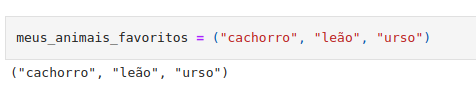
\includegraphics[scale=0.5]{imagens/tuplas01.png}
        \label{fig:my_label}
    \end{figure}    
\end{frame}

\begin{frame}{Estruturas de Dados}{Tuplas - Acesso}
    \begin{figure}
        \centering
        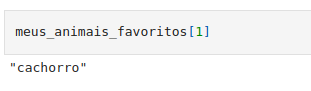
\includegraphics[scale=0.5]{imagens/tuplas02.png}
        \label{fig:my_label}
    \end{figure}    
\end{frame}

\begin{frame}{Estruturas de Dados}{Tuplas}
    \begin{itemize}
        \item Se tentamos mudar um elemento expecífico de uma tupla
    \end{itemize}
    \begin{figure}
        \centering
        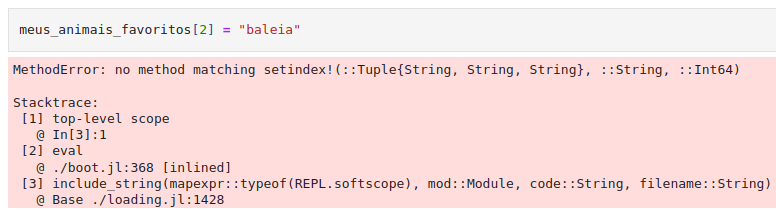
\includegraphics[scale=0.4]{imagens/tuplas03.png}
        \label{fig:my_label}
    \end{figure}
\end{frame}

\begin{frame}{Estruturas de Dados}{Tuplas}
    \begin{itemize}
        \item Podemos usar a palavra-chave ``in" para checar se um elemento pertence a uma tupla
    \end{itemize}
    \begin{figure}
        \centering
        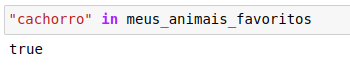
\includegraphics[scale=0.5]{imagens/tuplas05.png}
        \label{fig:my_label}
    \end{figure}
\end{frame}

\begin{frame}{Estruturas de Dados}{Tuplas-Nomeadas}
    \begin{itemize}
        \item Tuplas-Nomeadas são semelhantes a Tuplas 
        \item A exceção é que cada elemento tem um nome adicional
    \end{itemize}
\end{frame}

\begin{frame}{Estruturas de Dados}{Tuplas-Nomeadas}
    \begin{figure}
        \centering
        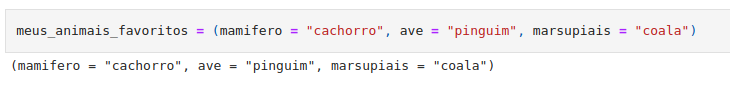
\includegraphics[scale=0.4]{imagens/tuplas-nomeadas01.png}
        \label{fig:my_label}
    \end{figure}
\end{frame}

\begin{frame}{Estruturas de Dados}{Tuplas-Nomeadas}
    \begin{itemize}
        \item Também podemos acessar os elementos via indexação
    \end{itemize}
    \begin{figure}
        \centering
        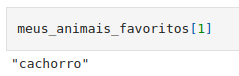
\includegraphics[scale=0.5]{imagens/tuplas-nomeadas02.png}
        \label{fig:my_label}
    \end{figure}
\end{frame}

\begin{frame}{Estruturas de Dados}{Tuplas-Nomeadas}
    \begin{itemize}
        \item Ganhamos uma nova maneira de acessar os elementos
    \end{itemize}
    \begin{figure}
        \centering
        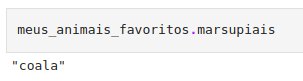
\includegraphics[scale=0.5]{imagens/tuplas-nomeadas03.png}
        \label{fig:my_label}
    \end{figure}
\end{frame}


\begin{frame}{Estruturas de Dados}{Dicionários}
    \begin{itemize}
        \item Usamos dicionários quando temos um conjunto de dados que se relacionam
        \item Um bom exemplo para um dicionário é a lista de contatos de emails
    \end{itemize}
\end{frame}

\begin{frame}{Estruturas de Dados}{Dicionários}
    \begin{figure}
        \centering
        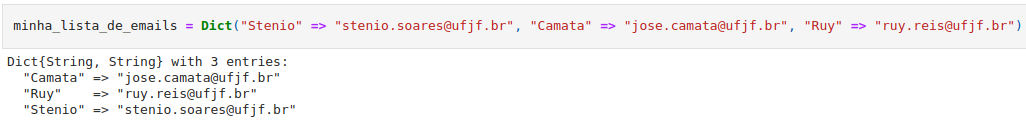
\includegraphics[scale=0.3]{imagens/dicionario01.png}
        \label{fig:my_label}
    \end{figure}
\end{frame}

\begin{frame}{Estruturas de Dados}{Dicionários}
    \begin{itemize}
        \item Podemos acessar nossos elementos por meio da sua chave
    \end{itemize}
    \begin{figure}
        \centering
        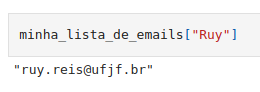
\includegraphics[scale=0.4]{imagens/dicionario02.png}
        \label{fig:my_label}
    \end{figure}
\end{frame}

\begin{frame}{Estruturas de Dados}{Dicionários}
    \begin{itemize}
        \item Podemos adicionar novos elementos no dicionário
    \end{itemize}
    \begin{figure}
        \centering
        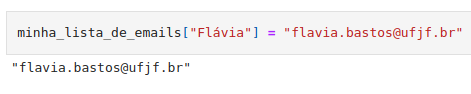
\includegraphics[scale=0.4]{imagens/dicionario03.png}
        \label{fig:my_label}
    \end{figure}
    \begin{figure}
        \centering
        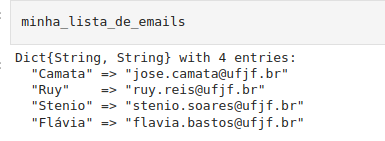
\includegraphics[scale=0.4]{imagens/dicionario04.png}
        \label{fig:my_label}
    \end{figure}
\end{frame}

\begin{frame}{Estruturas de Dados}{Dicionários}
    \begin{itemize}
        \item E também deletar elementos do dicionário
    \end{itemize}
    \begin{figure}
        \centering
        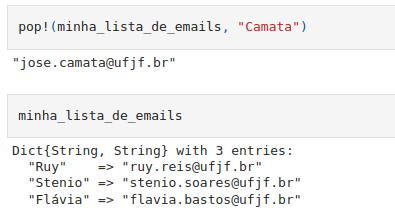
\includegraphics[scale=0.5]{imagens/dicionario05.png}
        \label{fig:my_label}
    \end{figure}
\end{frame}

\begin{frame}{Estruturas de Dados}{Dicionários}
    \begin{itemize}
        \item Ao contrário de Tuplas e Arrays, dicionários não são ordenados
        \item Assim, não conseguimos acessá-los por índices
    \end{itemize}
    \begin{figure}
        \centering
        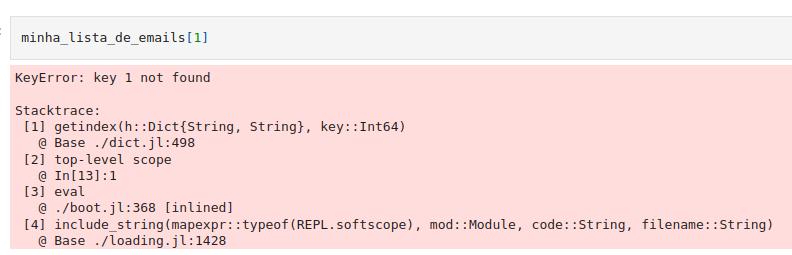
\includegraphics[scale=0.4]{imagens/dicionario06.png}
        \label{fig:my_label}
    \end{figure}
\end{frame}

\begin{frame}{Estruturas de Dados}{Dicionários}
    \begin{itemize}
        \item Assim como em dicionários da vida real, em Julia seguimos a ordem alfabética das chaves
    \end{itemize}
\end{frame}

\begin{frame}{Estruturas de Dados}{Arrays}
    \begin{itemize}
        \item Diferente de Tuplas, arrays são estruturas de dados mutáveis
        \item Diferente de dicionários, arrays contém coleções ordenadas
    \end{itemize}
\end{frame}

\begin{frame}{Estruturas de Dados}{Arrays - Declaração}
    \begin{figure}
        \centering
        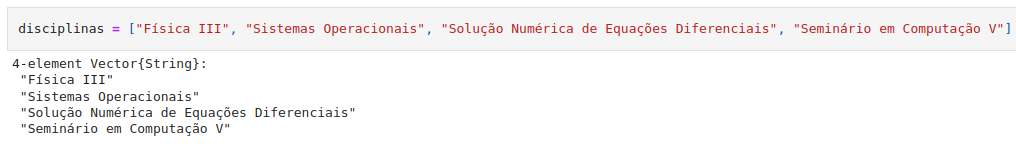
\includegraphics[scale=0.34]{imagens/array01.png}
        \label{fig:my_label}
    \end{figure}
\end{frame}

\begin{frame}{Estruturas de Dados}{Arrays - Declaração}
    \begin{figure}
        \centering
        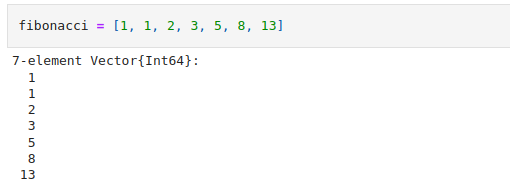
\includegraphics[scale=0.5]{imagens/array02.png}
        \label{fig:my_label}
    \end{figure}
\end{frame}

\begin{frame}{Estruturas de Dados}{Arrays - Declaração}
    \begin{figure}
        \centering
        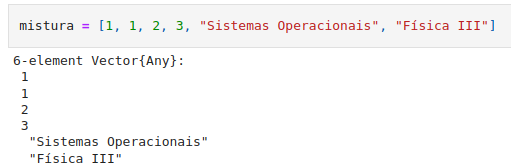
\includegraphics[scale=0.5]{imagens/array03.png}
        \label{fig:my_label}
    \end{figure}
\end{frame}

\begin{frame}{Estruturas de Dados}{Arrays - Manipulação}
    \begin{itemize}
        \item Uma vez declarado, podemos acessar um elemento específico do array
    \end{itemize}
    \begin{figure}
        \centering
        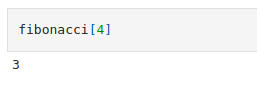
\includegraphics[scale=0.5]{imagens/array04.png}
        \label{fig:my_label}
    \end{figure}
\end{frame}

\begin{frame}{Estruturas de Dados}{Arrays - Manipulação}
    \begin{itemize}
        \item Podemos também manipular seus elementos
    \end{itemize}
    \begin{figure}
        \centering
        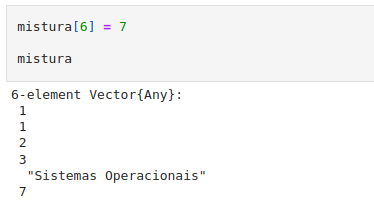
\includegraphics[scale=0.5]{imagens/array05.png}
        \label{fig:my_label}
    \end{figure}
\end{frame}

\begin{frame}{Estruturas de Dados}{Arrays - Manipulação}
    \begin{figure}
        \centering
        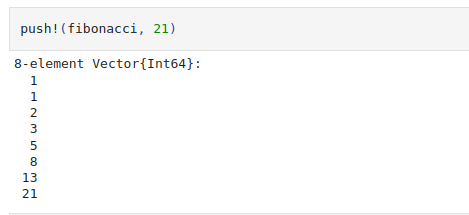
\includegraphics[scale=0.5]{imagens/array07.png}
        \label{fig:my_label}
    \end{figure}
\end{frame}

\begin{frame}{Estruturas de Dados}{Arrays - Manipulação}
    \begin{figure}
        \centering
        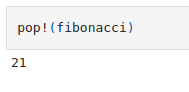
\includegraphics[scale=0.5]{imagens/array08.png}
        \label{fig:my_label}
    \end{figure}
\end{frame}

\begin{frame}{Estruturas de Dados}{Arrays Multidimensionais}
    \begin{itemize}
        \item Até agora trabalhamos com arrays unidimensionais
        \item Julia também nos permite trabalhar com arrays com um número arbitrário de dimensões
    \end{itemize}
\end{frame}

\begin{frame}{Estruturas de Dados}{Arrays Multidimensionais}
    \begin{figure}
        \centering
        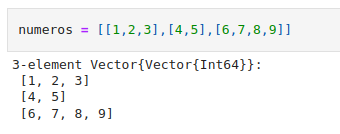
\includegraphics[scale=0.5]{imagens/array09.png}
        \label{fig:my_label}
    \end{figure}
\end{frame}

\begin{frame}{Estruturas de Dados}{Arrays Multidimensionais}
    \begin{itemize}
        \item Também podemos inicializar aleatoriamente nossos arrays
    \end{itemize}
\end{frame}


\begin{frame}{Estruturas de Dados}{Arrays Multidimensionais}
    \begin{figure}
        \centering
        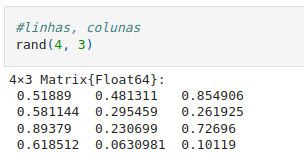
\includegraphics[scale=0.5]{imagens/array10.png}
        \label{fig:my_label}
    \end{figure}
\end{frame}

\begin{frame}{Estruturas de Dados}{Arrays Multidimensionais}
    \begin{figure}
        \centering
        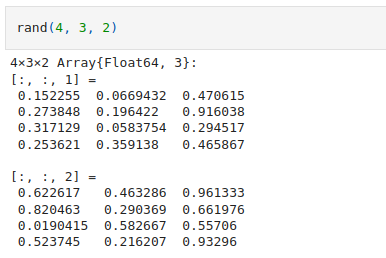
\includegraphics[scale=0.5]{imagens/array11.png}
        \label{fig:my_label}
    \end{figure}
\end{frame}

\begin{frame}{Estruturas de Dados}{Arrays - Cópias}
    \begin{itemize}
        \item Temos que ter muito cuidado ao fazer cópias de arrays
    \end{itemize}
\end{frame}

\begin{frame}{Estruturas de Dados}{Arrays - Cópias}
    \begin{figure}
        \centering
        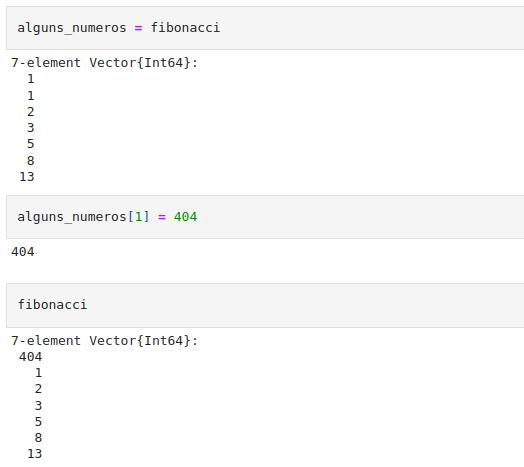
\includegraphics[scale=0.4]{imagens/array12.png}
        \label{fig:my_label}
    \end{figure}
\end{frame}

\begin{frame}{Estruturas de Dados}{Arrays - Cópias}
    \begin{figure}
        \centering
        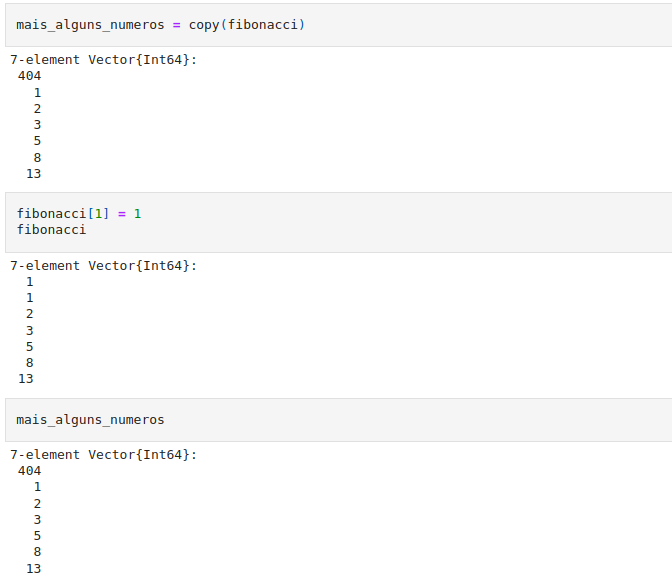
\includegraphics[scale=0.3]{imagens/array13.png}
        \label{fig:my_label}
    \end{figure}
\end{frame}

\section{Condicionais e Estruturas de Repetição}

\begin{frame}{Blocos de identação}
    \begin{itemize}
        \item Ao contrário de linguagens como C, C++ e Java, Julia não tem blocos de identação
        \item Sua ``orientação" é bem parecida com a sintaxe do Matlab, onde não há uma obrigatoriedade de identar seu código
    \end{itemize}
\end{frame}

\begin{frame}{Blocos de identação}
    \begin{itemize}
        \item Mas lembre-se: ``Um código bem identado é um código mais legível!"
    \end{itemize}
\end{frame}

\begin{frame}{Condicionais}{Sintaxe}
    \begin{itemize}
        \item Como em várias linguagens, fazemos condicionais com a palavra-chave \textit{if}
    \end{itemize}
    \begin{figure}
        \centering
        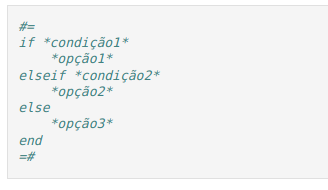
\includegraphics[scale=0.4]{imagens/if-sintaxe.png}
        \label{fig:my_label}
    \end{figure}
\end{frame}

\begin{frame}{Condicionais}{Sintaxe}
    \begin{itemize}
        \item Condicionais com a sintaxe acima nos permitem avaliar condicionalmente expressões
        \item Um bom caso para exemplo é o \textit{Teste FizzBuzz}
    \end{itemize}
\end{frame}

\begin{frame}{Condicionais}{Exemplo - Teste FizzBuzz}
    \textbf{Dado um número, N, imprima "Fizz" se N é divisível por $3$ , "Buzz" se N é divisível por $5$ e "FizzBuzz" se  é divisível por $3$ e $5$ ao mesmo tempo. Se nenhuma das condições for atendida, apenas imprima o número fornecido.}
\end{frame}

\begin{frame}{Condicionais}{Exemplo - Teste FizzBuzz}
     \begin{figure}
        \centering
        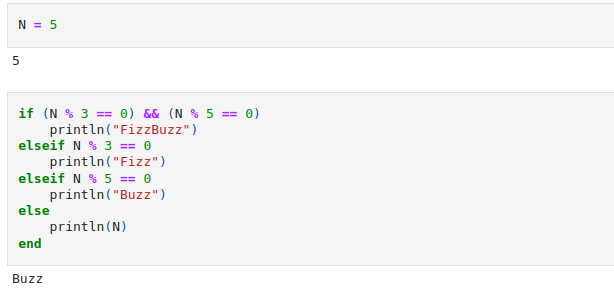
\includegraphics[scale=0.5]{imagens/teste-fizzbuzz.png}
        \label{fig:my_label}
    \end{figure}   
\end{frame}

\begin{frame}{Condicionais}{Operadores ternários}
    \begin{itemize}
        \item Assim como em outras linguagens, Julia nos permite usar \textbf{operadores ternários}
        \item Funciona com o mesmo conceito que o \textit{if...else}
        \item Obrigatoriamente precisamos devolver um valor após o teste
        \item Só é válido para operações que podem ser implementadas em uma única linha 
    \end{itemize}
\end{frame}

\begin{frame}{Condicionais}{Operadores ternários - Exemplo}
    \begin{itemize}
        \item Se temos as seguintes variáveis
    \end{itemize}
    \begin{figure}
        \centering
        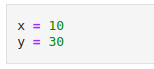
\includegraphics[scale=0.5]{imagens/var-if.png}
        \label{fig:my_label}
    \end{figure}  
\end{frame}

\begin{frame}{Condicionais}{Operadores ternários - Exemplo}
    \begin{itemize}
        \item Um código simples para saber qual delas é maior pode ser escrito com
    \end{itemize}
    \begin{figure}
        \centering
        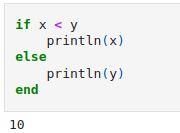
\includegraphics[scale=0.5]{imagens/if-002.png}
        \label{fig:my_label}
    \end{figure}  
\end{frame}

\begin{frame}{Condicionais}{Operadores ternários - Exemplo}
    \begin{itemize}
        \item Imagine que seu chefe te deu a seguinte ordem:
        \begin{center}
            ``Você tem $R\$15000,00$ para esse projeto. A cada linha que vc escreve $R\$5,00$ são tirados do orçamento. Você tem que escrever todo o código de qualquer maneira, e se faltar orçamento, sai do seu salário!"
        \end{center}
    \end{itemize}
\end{frame}

\begin{frame}{Condicionais}{Operadores ternários - Exemplo}
    \begin{itemize}
        \item Para não perdermos orçamento, e, provavelmente salário, podemos fazer o uso de Operadores Ternários
    \end{itemize}
\end{frame}

\begin{frame}{Condicionais}{Operadores ternários - Exemplo}
    \begin{figure}
        \centering
        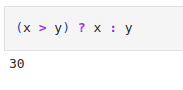
\includegraphics[scale=0.6]{imagens/ternario.png}
        \label{fig:my_label}
    \end{figure}  
\end{frame}

\begin{frame}{Condicionais}{Operadores ternários - Exemplo}
    \begin{itemize}
        \item Economizamos $4$ linhas de código
        \item Claro que esse foi um exemplo bobo e não real
        \item Mas operadores ternários são bem úteis no dia-a-dia
    \end{itemize}
\end{frame}

\begin{frame}{Estruturas de repetição}{Sintaxe}
    \begin{figure}
        \centering
        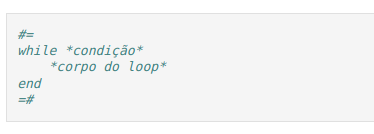
\includegraphics[scale=0.6]{imagens/while.png}
        \label{fig:my_label}
    \end{figure}
\end{frame}

\begin{frame}{Estruturas de repetição}{Sintaxe}
    \begin{figure}
        \centering
        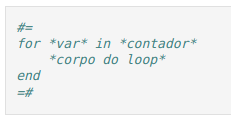
\includegraphics[scale=0.6]{imagens/for.png}
        \label{fig:my_label}
    \end{figure}
\end{frame}

\begin{frame}{Estruturas de repetição}{Exemplo}
    \begin{figure}
        \centering
        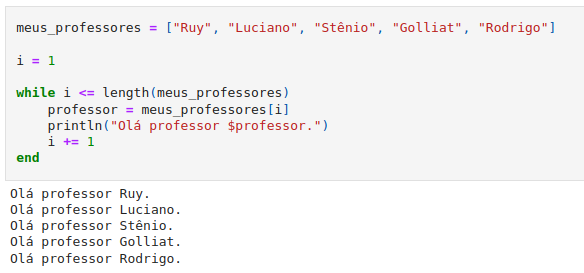
\includegraphics[scale=0.4]{imagens/ex-while.png}
        \label{fig:my_label}
    \end{figure}
\end{frame}

\begin{frame}{Estruturas de repetição}{Exemplo}
    \begin{figure}
        \centering
        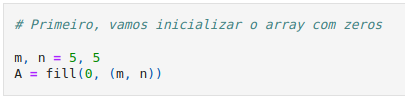
\includegraphics[scale=0.4]{imagens/matriz-zerada.png}
        \label{fig:my_label}
    \end{figure}
    \begin{figure}
        \centering
        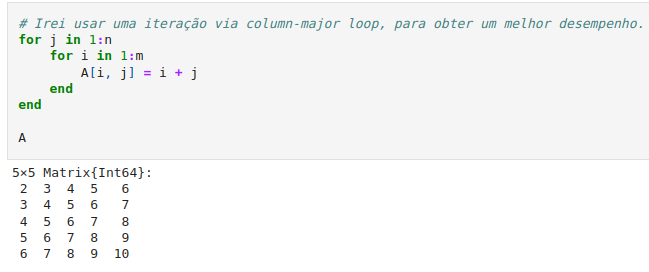
\includegraphics[scale=0.4]{imagens/ex-for.png}
        \label{fig:my_label}
    \end{figure}
\end{frame}

\begin{frame}{Exercício}
    \textbf{Crie uma matriz antissimétrica de ordem $5$. Após isso, imprima a matriz}.
\end{frame}

\begin{frame}{Exercício}{Gabarito}
    \begin{figure}
        \centering
        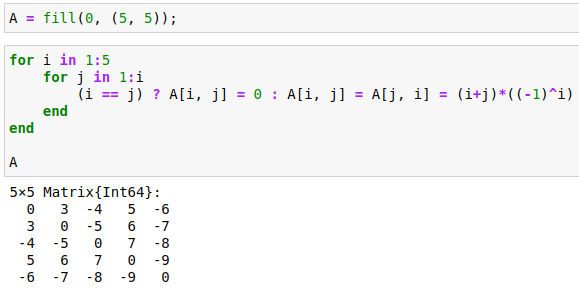
\includegraphics[scale=0.4]{imagens/gabarito-ex01.png}
        \label{fig:my_label}
    \end{figure}    
\end{frame}


\section{Funções e Structs}
\begin{frame}{Funções}{Como declarar uma função}
    \begin{itemize}
        \item Em Julia, podemos declarar funções de algumas maneiras diferentes
        \item A primeira e mais comum irá requerer as palavras-chave \textit{function} e \textit{end}
    \end{itemize}
\end{frame}

\begin{frame}{Funções}{Como declarar uma função}
    \begin{figure}
        \centering
        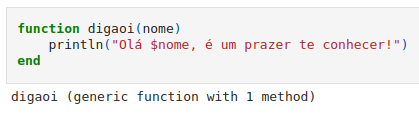
\includegraphics[scale=0.4]{imagens/func01.png}
        \label{fig:my_label}
    \end{figure}   
\end{frame}

\begin{frame}{Funções}{Como declarar uma função}
    \begin{figure}
        \centering
        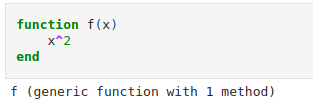
\includegraphics[scale=0.4]{imagens/func02.png}
        \label{fig:my_label}
    \end{figure}   
\end{frame}

\begin{frame}{Funções}{Como declarar uma função}
    \begin{itemize}
        \item Podemos chamar nossas funções da seguinte maneira
    \end{itemize}
    \begin{figure}
        \centering
        \includegraphics[scale=0.4]{imagens/func03.png}
        \label{fig:my_label}
    \end{figure}   
\end{frame}

\begin{frame}{Funções}{\textit{Duck-typing}}
    \begin{center}
        \textbf{``If it quacks like a duck, walks like a duck and looks like a duck, IT'S A DUCK!"}
    \end{center} 
\end{frame}

\begin{frame}{Funções}{\textit{Duck-typing}}
    \begin{itemize}
        \item Nesse tipo de função o compilador irá trabalhar apenas com as entradas que fazem algum sentido
        \item Por exemplo, nossa função \textit{digaoi()} funciona com qualquer tipo de dado
    \end{itemize}
    \begin{figure}
        \centering
        \includegraphics[scale=0.4]{imagens/abs.png}
        \label{fig:my_label}
    \end{figure}     
\end{frame}

\begin{frame}{Funções}{\textit{Duck-typing}}
    \begin{itemize}
        \item A função \textit{f()} também funciona com matrizes
    \end{itemize}
    \begin{figure}
        \centering
        \includegraphics[scale=0.4]{imagens/mat-ex-func.png}
        \label{fig:my_label}
    \end{figure}     
\end{frame}

\begin{frame}{Funções}{\textit{Duck-typing}}
    \begin{itemize}
        \item Isso acontece pois $A^2$ é algo bem definido
        \item O que não acontece por exemplo com um vetor
    \end{itemize}
    \begin{figure}
        \centering
        \includegraphics[scale=0.4]{imagens/vet-ex-func.png}
        \label{fig:my_label}
    \end{figure}     
\end{frame}

\begin{frame}{Structs}{Sintaxe}
    \begin{figure}
        \centering
        \includegraphics[scale=0.4]{imagens/struct-ex.png}
        \label{fig:my_label}
    \end{figure}     
\end{frame}

\begin{frame}{Structs}{Sintaxe}
    \begin{figure}
        \centering
        \includegraphics[scale=0.4]{imagens/struct-ex02.png}
        \label{fig:my_label}
    \end{figure}     
\end{frame}

\begin{frame}{Structs}{Sintaxe}
    \begin{figure}
        \centering
        \includegraphics[scale=0.4]{imagens/struct-ex03.png}
        \label{fig:my_label}
    \end{figure}     
\end{frame}

\begin{frame}{Structs}{Sintaxe}
    \begin{figure}
        \centering
        \includegraphics[scale=0.4]{imagens/struct-ex04.png}
        \label{fig:my_label}
    \end{figure}     
\end{frame}

\begin{frame}{Structs}{Sintaxe}
    \begin{figure}
        \centering
        \includegraphics[scale=0.4]{imagens/struct-ex06.png}
        \label{fig:my_label}
    \end{figure}     
\end{frame}


\section{Bibliotecas}

\begin{frame}{Bibliotecas}{Pacotes}
    \begin{itemize}
        \item Julia tem mais de $2000$ pacotes registrados
        \item A maioria dos pacotes estão registrados no próprio site da linguagem \footnote{https://julialang.org/packages/}
    \end{itemize}
\end{frame}

\begin{frame}{Bibliotecas}{Instalando pacotes}
    A primeira vez que usamos um pacote em uma instalação nova da linguagem Julia, precisamos pedir ao gerenciador de pacores que adicione-o explicitamente
    \begin{figure}
        \centering
        \includegraphics[scale=0.34]{imagens/pacotes-ex01.png}
        \label{fig:my_label}
    \end{figure}
\end{frame}

\begin{frame}{Bibliotecas}{Exemplo}
    Um pacote legal para brincar é o ``Colors"
    \begin{figure}
        \centering
        \includegraphics[scale=0.34]{imagens/colors.png}
        \label{fig:my_label}
    \end{figure}
\end{frame}

\begin{frame}{Bibliotecas}{Exemplo}
    \begin{figure}
        \centering
        \includegraphics[scale=0.34]{imagens/colors-02.png}
        \label{fig:my_label}
    \end{figure}
    \begin{figure}
        \centering
        \includegraphics[scale=0.3]{imagens/colors-03.png}
        \label{fig:my_label}
    \end{figure}
    \begin{figure}
        \centering
        \includegraphics[scale=0.3]{imagens/colors04.png}
        \label{fig:my_label}
    \end{figure}
\end{frame}


\begin{frame}{Bibliotecas}{Plot}
    Vamos ver agora como trabalhar com plots em Julia. Primeiro, temos que importar o pacote ``Plots"
    \begin{figure}
        \centering
        \includegraphics[scale=0.5]{imagens/plot.png}
        \label{fig:my_label}
    \end{figure}
\end{frame}

\begin{frame}{Bibliotecas}{Plot}
    \begin{figure}
        \centering
        \includegraphics[scale=0.5]{imagens/plot02.png}
        \label{fig:my_label}
    \end{figure}
\end{frame}

\begin{frame}{Bibliotecas}{Plot}
    \begin{figure}
        \centering
        \includegraphics[scale=0.4]{imagens/plot03.png}
        \label{fig:my_label}
    \end{figure}
\end{frame}

\begin{frame}{Bibliotecas}{Plot}
    \begin{figure}
        \centering
        \includegraphics[scale=0.35]{imagens/plot04.png}
        \label{fig:my_label}
    \end{figure}
\end{frame}

\begin{frame}{Bibliotecas}{Plot}
    \begin{figure}
        \centering
        \includegraphics[scale=0.4]{imagens/plot05.png}
        \label{fig:my_label}
    \end{figure}
\end{frame}

\begin{frame}{Bibliotecas}{Plot}
    \begin{figure}
        \centering
        \includegraphics[scale=0.4]{imagens/plot06.png}
        \label{fig:my_label}
    \end{figure}
\end{frame}

\section*{Exercícios de aplicação}

\begin{frame}{Exercício Geral}
    \begin{center}
        \textbf{Crie um programa que seja capaz de cadastrar pessoas em uma loja de peças eletrônicas. A cada compra que uma pessoa faz, ela recebe o valor do produto em pontos de fidelidade. Quando a pessoa atinge $7000$ pontos, ela tem direito a um desconto de $15\%$ na próxima compra. O programa deve receber o nome da pessoa, checar se ela já é cadastrada e, se for, adicionar os pontos em seu cadastro; se não, deve criar o cadastro. O programa deve receber valores dos produtos da compra até que seja digitado o valor $-1$. Se a pessoa chegar na quantidade de pontos necessária para ganhar o desconto, o mesmo deve ser aplicado no valor final da compra.}
    \end{center}
\end{frame}

\begin{frame}{Próximos passos...}
    \begin{itemize}
        \item Cursos mais focados em áreas específicas podem ser achados na Julia Academy
        \item Treinar e escrever projetos maiores na linguagem
        \item Reescrever sistemas feitos em Python e Matlab em Julia
    \end{itemize}
\end{frame}

\begin{frame}{Contato}
    \begin{center}
        \textcolor{blue}{\textbf{João Víctor Costa de Oliveira:}} joao.oliveira@ice.ufjf.br\\
    \end{center}
\end{frame}



\end{document}

